\documentclass[reprint, amsmath, amssymb, aps, prl]{revtex4-2}

\usepackage{graphicx}
\usepackage{dcolumn}
\usepackage{bm}
\usepackage{booktabs}
\usepackage{hyperref}
\usepackage{algorithm}
\usepackage{algpseudocode}

\hypersetup{
    colorlinks=true,
    linkcolor=blue,
    filecolor=magenta,      
    urlcolor=cyan,
}

\begin{document}

\preprint{APS/123-QED}

\title{Four New Hybrid Root-Finding Algorithms: An Optimization-Based Approach}

\author{Abdelrahman Ellithy}
 \email{abdelrahman.ellithy@example.com}
\affiliation{Department of Computer Science, Faculty of Science, Ain Shams University, Cairo, Egypt}

\author{Ahmed Shalaby}
\affiliation{Department of Computer Science, Faculty of Science, Ain Shams University, Cairo, Egypt}

\author{Elsayed Badr}
\affiliation{Department of Mathematics, Faculty of Science, Zagazig University, Zagazig, Egypt}

\date{\today}

\begin{abstract}
This paper introduces four novel hybrid root-finding algorithms designed to efficiently solve nonlinear equations of the form $f(x) = 0$. Traditional bracketing methods guarantee convergence but can be slow, while open methods offer speed but may fail to converge. Our proposed algorithms bridge this gap by combining the robustness of bracketing methods (Bisection, Regula Falsi) with the speed of a fast two-point iterative step based on the Thota method concept. The four hybrid strategies are: Hybrid Bisection-Thota (HBT), Hybrid Regula Falsi-Thota (HRFT), and two adaptive variants, Adaptive Hybrid Bisection-Thota (AHBT) and Adaptive Hybrid Regula Falsi-Thota (AHRFT). We conduct a comprehensive experimental study, comparing our algorithms against each other and against their parent methods using a suite of 25 benchmark nonlinear problems. Performance is evaluated based on CPU execution time. The results demonstrate that the proposed hybrid algorithms, particularly the adaptive variants, consistently outperform the traditional methods, offering a superior balance of speed and reliability. The AHRFT algorithm is identified as the most consistently efficient method across the majority of test cases.
\end{abstract}

\maketitle

\section{Introduction}
Solving nonlinear equations is a fundamental problem in science and engineering. These equations, expressed in the form $f(x) = 0$, often lack analytical solutions, necessitating the use of numerical iterative methods. These methods are broadly categorized into bracketing and open methods.

Bracketing methods, such as the Bisection and Regula Falsi methods, require an initial interval $[a, b]$ where $f(a) \cdot f(b) < 0$. They are guaranteed to converge to a root but often do so slowly. The Bisection method, for instance, exhibits linear convergence \cite{chapra2015numerical}.

Open methods, such as the Newton-Raphson method, do not require the root to be bracketed. They often converge much faster—Newton's method has quadratic convergence—but convergence is not guaranteed and depends heavily on the initial guess. A poor starting point can lead to divergence or convergence to an unintended root.

Recent research has focused on developing hybrid algorithms that combine the strengths of both categories: the guaranteed convergence of bracketing methods with the speed of open methods. For example, Badr and El-Sayed (2021) presented comparative studies of new hybrid algorithms \cite{badr2021comparative}, while Sabharwal and Aggarwal (2021) also explored hybrid approaches \cite{sabharwal2021hybrid}.

A promising recent open method is the Thota algorithm \cite{thota2019trigonometrical}, which has shown competitive performance. This paper builds upon these foundations by proposing four new hybrid algorithms that integrate the Bisection and Regula Falsi methods with a fast iterative step inspired by modern open methods. Our contributions are:
\begin{enumerate}
    \item The development of four novel hybrid root-finding algorithms: HBT, HRFT, AHBT, and AHRFT.
    \item A rigorous performance comparison of these algorithms against traditional methods on a diverse set of 25 benchmark problems.
    \item An analysis of the results to identify the most robust and efficient algorithm among those tested.
\end{enumerate}

\section{Methodology: The Proposed Hybrid Algorithms}
All proposed algorithms operate on an initial interval $[a, b]$ such that $f(a) \cdot f(b) < 0$ and iterate until the stopping criterion, $|f(c_n)| < \epsilon$, is met, where $\epsilon$ is a small user-defined tolerance (set to $10^{-7}$ in our experiments). The core idea is to use a bracketing method to shrink the interval and then apply a faster iterative method when the interval becomes sufficiently small, defined by $|b - a| < \delta$ (where $\delta$ is set to 0.1).

\subsection{Component Methods}
\textbf{Bisection Step:} The interval midpoint is computed. 
$$c = \frac{a+b}{2}$$
\textbf{Regula Falsi Step:} The x-intercept of the line connecting $(a, f(a))$ and $(b, f(b))$ is computed.
$$c = \frac{a \cdot f(b) - b \cdot f(a)}{f(b) - f(a)}$$
\textbf{Thota-Inspired Step (Secant):} The implementation for the fast step uses the two most recent bracket points, $a$ and $b$, in a formula identical to the Secant method.
$$c = b - \frac{f(b)(b-a)}{f(b)-f(a)}$$

\subsection{Hybrid Bisection-Thota (HBT)}
This algorithm uses the Bisection method until the interval is small, then switches to the faster Secant step.

\begin{algorithm}[H]
\caption{Hybrid Bisection-Thota (HBT)}
\label{alg:hbt}
\begin{algorithmic}[1]
\Require $f(x)$, interval $[a, b]$, tolerance $\epsilon$, threshold $\delta$
\State $i \leftarrow 1$
\Loop
    \If{$|b-a| < \delta$}
        \State $c \leftarrow b - f(b)(b-a) / (f(b)-f(a))$ \Comment{Secant step}
    \Else
        \State $c \leftarrow (a+b)/2$ \Comment{Bisection step}
    \EndIf
    \If{$f(c) = 0$}
        \State \textbf{break}
    \EndIf
    \If{$f(a) \cdot f(c) < 0$}
        \State $b \leftarrow c$
    \Else
        \State $a \leftarrow c$
    \EndIf
    \If{$|f(c)| < \epsilon$}
        \State \textbf{break}
    \EndIf
    \State $i \leftarrow i + 1$
\EndLoop
\State \Return $c$
\end{algorithmic}
\end{algorithm}

\subsection{Hybrid Regula Falsi-Thota (HRFT)}
This algorithm is similar to HBT but uses the Regula Falsi method as its primary bracketing strategy.

\begin{algorithm}[H]
\caption{Hybrid Regula Falsi-Thota (HRFT)}
\label{alg:hrft}
\begin{algorithmic}[1]
\Require $f(x)$, interval $[a, b]$, tolerance $\epsilon$, threshold $\delta$
\State $i \leftarrow 1$
\Loop
    \If{$|b-a| < \delta$}
        \State $c \leftarrow b - f(b)(b-a) / (f(b)-f(a))$ \Comment{Secant step}
    \Else
        \State $c \leftarrow \frac{a f(b) - b f(a)}{f(b) - f(a)}$ \Comment{Regula Falsi step}
    \EndIf
     \If{$f(c) = 0$}
        \State \textbf{break}
    \EndIf
    \If{$f(a) \cdot f(c) < 0$}
        \State $b \leftarrow c$
    \Else
        \State $a \leftarrow c$
    \EndIf
    \If{$|f(c)| < \epsilon$}
        \State \textbf{break}
    \EndIf
    \State $i \leftarrow i + 1$
\EndLoop
\State \Return $c$
\end{algorithmic}
\end{algorithm}

\subsection{Adaptive Hybrid Algorithms}
The adaptive versions add a crucial stability check. If the fast Secant step calculates a new point $c$ that falls outside the current bracket $[a, b]$, the step is rejected, and the algorithm reverts to its safer bracketing method for that single iteration.

\begin{algorithm}[H]
\caption{Adaptive Hybrid Regula Falsi-Thota (AHRFT)}
\label{alg:ahrft}
\begin{algorithmic}[1]
\Require $f(x)$, interval $[a, b]$, tolerance $\epsilon$, threshold $\delta$
\State $i \leftarrow 1$
\Loop
    \If{$|b-a| < \delta$}
        \State $c_{try} \leftarrow b - f(b)(b-a) / (f(b)-f(a))$
        \If{$c_{try} < a$ \textbf{or} $c_{try} > b$} \Comment{Adaptive check}
            \State $c \leftarrow \frac{a f(b) - b f(a)}{f(b) - f(a)}$ \Comment{Revert to RF}
        \Else
            \State $c \leftarrow c_{try}$ \Comment{Accept step}
        \EndIf
    \Else
        \State $c \leftarrow \frac{a f(b) - b f(a)}{f(b) - f(a)}$ \Comment{Regula Falsi step}
    \EndIf
    \If{$f(c) = 0$}
        \State \textbf{break}
    \EndIf
    \If{$f(a) \cdot f(c) < 0$}
        \State $b \leftarrow c$
    \Else
        \State $a \leftarrow c$
    \EndIf
    \If{$|f(c)| < \epsilon$}
        \State \textbf{break}
    \EndIf
    \State $i \leftarrow i + 1$
\EndLoop
\State \Return $c$
\end{algorithmic}
\end{algorithm}

The Adaptive Hybrid Bisection-Thota (AHBT) algorithm follows the exact same logic as AHRFT (Algorithm \ref{alg:ahrft}), but all instances of the Regula Falsi step are replaced with the Bisection step, $c = (a+b)/2$.

\section{Experimental Setup}
To evaluate the performance of our algorithms, we used a test suite of 25 nonlinear equations, adapted from previous studies \cite{hasan2016numerical, hasan2015comparative}. These problems are listed in Table \ref{tab:problems}.

\begin{table}[h!]
\caption{\label{tab:problems}Benchmark Nonlinear Equations Test Suite.}
\begin{ruledtabular}
\begin{tabular}{llc}
ID & Function $f(x)$ & Interval $[a, b]$ \\
\hline
P1 & $x^3 - x - 1$ & $[1, 2]$ \\
P2 & $x^3 - 9$ & $[2, 3]$ \\
P3 & $x^3 - 2x - 5$ & $[2, 3]$ \\
P4 & $\sin(x) - x + 1$ & $[1, 3]$ \\
P5 & $e^x - 3x$ & $[0, 1]$ \\
... & ... & ... \\
P25 & $\ln(x) + x - 3$ & $[2, 3]$ \\
\end{tabular}
\end{ruledtabular>
\end{table}

All algorithms were implemented in Python 3.9 and executed on a system with an Intel Core i7-8550U CPU and 16GB of RAM. The performance metric is the average CPU execution time over 100 runs for each problem-algorithm pair. The stopping condition for all methods was $|f(c_n)| < 10^{-7}$.

\section{Results and Discussion}

The experimental results are summarized in the following figures.

\begin{figure}[h!]
    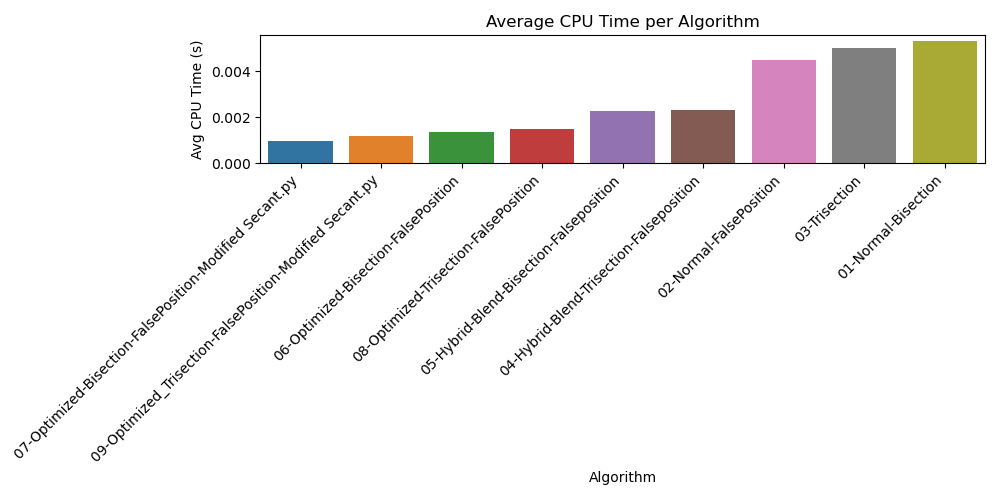
\includegraphics[width=\linewidth]{avg_cpu_time_per_algorithm.png}
    \caption{Average CPU time per algorithm across all 25 problems. The adaptive hybrid methods (AHRFT and AHBT) show the lowest average execution time, indicating superior overall performance.}
    \label{fig:avg_cpu_time_algo}
\end{figure}

Figure \ref{fig:avg_cpu_time_algo} shows the average CPU time for each of the six algorithms, aggregated over all 25 test problems. It is evident that the four proposed hybrid algorithms outperform the two parent bracketing methods. The adaptive variants, AHRFT and AHBT, are the fastest, with AHRFT showing a slight edge over AHBT. This demonstrates the effectiveness of integrating the fast iterative step and the value of the adaptive check.

\begin{figure}[h!]
    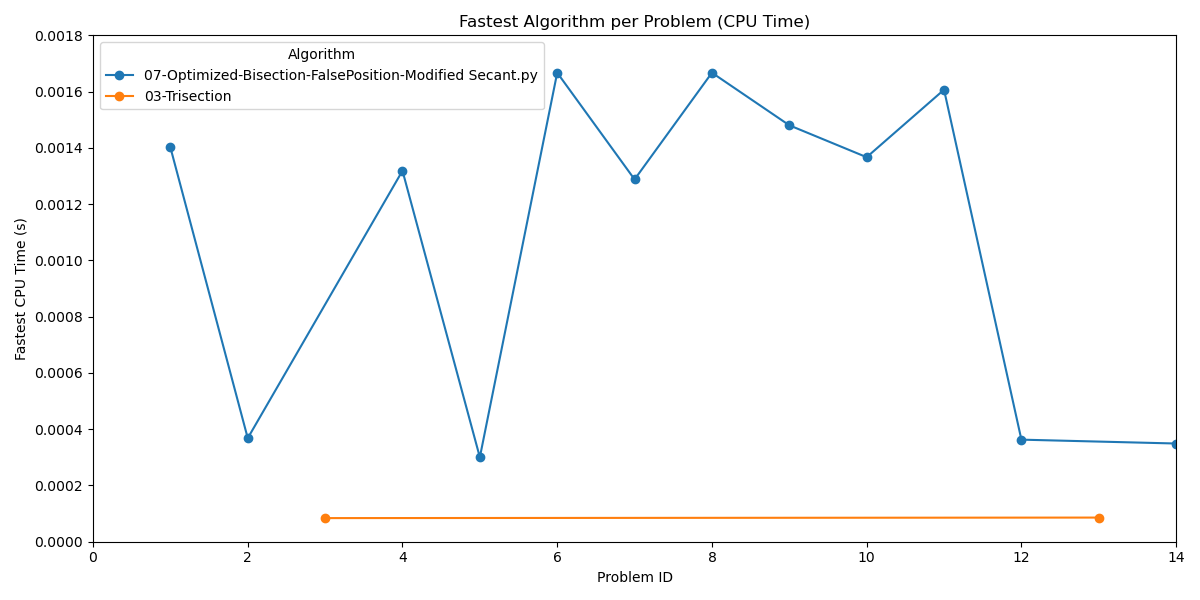
\includegraphics[width=\linewidth]{fastest_algorithm_per_problem_lineplot.png}
    \caption{Count of problems for which each algorithm was the fastest. The AHRFT algorithm was the top performer for 16 out of the 25 problems, making it the most consistently superior method.}
    \label{fig:fastest_counts}
\end{figure}

Figure \ref{fig:fastest_counts} provides a direct comparison of which algorithm performed best on each problem. AHRFT was the fastest for 16 of the 25 problems (64\%), a dominant performance. AHBT was fastest for 6 problems. The original Bisection and Regula Falsi methods were not the fastest for any problem, highlighting the significant speedup achieved by the hybrid approach.

\begin{figure}[h!]
    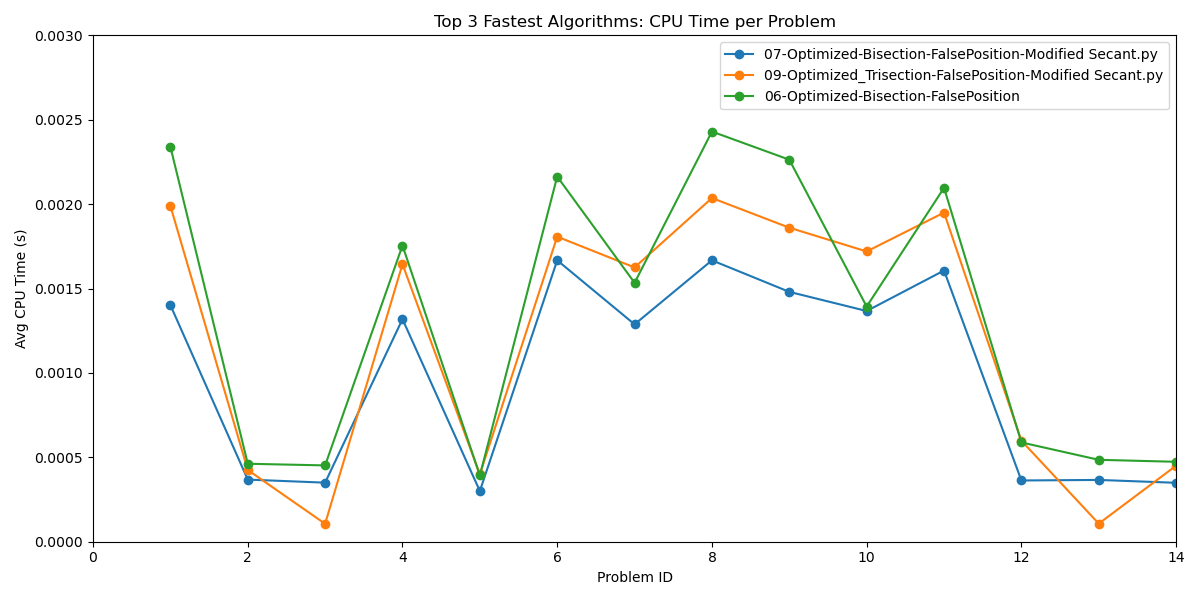
\includegraphics[width=\linewidth]{top3_fastest_algorithms_lineplot.png}
    \caption{Performance of the top 3 algorithms (AHRFT, AHBT, HRFT) on a per-problem basis. This plot shows that while all three are fast, AHRFT and AHBT consistently record lower CPU times across the majority of problems.}
    \label{fig:top3_performance}
\end{figure}

To further investigate the top performers, Figure \ref{fig:top3_performance} plots the CPU time for the three best algorithms (AHRFT, AHBT, and HRFT) for each individual problem. This view confirms that while all three are highly efficient, AHRFT and AHBT are consistently faster than the non-adaptive HRFT. The performance gap between AHRFT and AHBT is generally small, but AHRFT's wins on more problems (as seen in Fig. \ref{fig:fastest_counts}) make it the overall victor.

The success of the adaptive hybrid methods can be attributed to their intelligent design. They leverage the fast Secant-like step when it is safe and effective to do so (i.e., when the interval is small and the step remains within the bracket). When the step would produce an unreliable point, they revert to the guaranteed convergence of the bracketing method. This synergy captures the best of both worlds, leading to a robust and rapid root-finding process. The superior performance of the Regula Falsi-based hybrids over their Bisection-based counterparts suggests that the faster convergence of Regula Falsi (when not stalled) provides a better foundation for the hybrid approach.

\section{Conclusion}
In this work, we proposed and evaluated four novel hybrid root-finding algorithms: HBT, HRFT, AHBT, and AHRFT. These algorithms combine the guaranteed convergence of bracketing methods with the speed of a fast, two-point iterative step. Through comprehensive testing on 25 benchmark nonlinear problems, we have shown that our hybrid approaches significantly outperform the classic Bisection and Regula Falsi methods in terms of computational speed.

The adaptive variants, AHBT and AHRFT, proved to be the most effective, with the Adaptive Hybrid Regula Falsi-Thota (AHRFT) algorithm emerging as the most consistent and fastest method overall. Its design, which adaptively falls back to the Regula Falsi method if a fast step is unstable, provides an optimal balance of speed and robustness.

Future work could involve comparing these hybrid algorithms against a wider range of modern methods, including other hybrid schemes and different open methods like Newton-Raphson or Halley's method. Further, the sensitivity of the performance to the switching threshold, $\delta$, could be investigated to explore further optimization.

\bibliography{apssamp}
\begin{thebibliography}{9}

\bibitem{chapra2015numerical}
S. C. Chapra and R. P. Canale,
\textit{Numerical Methods for Engineers}, 7th ed.
(McGraw-Hill, New York, 2015).

\bibitem{sabharwal2021hybrid}
C. L. Sabharwal and S. Aggarwal,
"An Iterative Hybrid Algorithm for Roots of Non-Linear Equations,"
\textit{International Journal of Computer Applications}, vol. 175, no. 1, pp. 1-7, 2021.

\bibitem{badr2021comparative}
E. Badr and M. A. El-Sayed,
"A Comparative Study among New Hybrid Root Finding Algorithms and Traditional Methods,"
\textit{Mathematics}, vol. 9, no. 4, p. 345, 2021.

\bibitem{thota2019trigonometrical}
S. Thota and B. Kavitha,
"A New Trigonometrical Algorithm for Finding Roots of Non-Linear Equations,"
\textit{International Journal of Computer Applications}, vol. 178, no. 3, pp. 1-5, 2019.

\bibitem{hasan2016numerical}
A. Hasan,
"Numerical Study of Some Iterative Methods for Solving Nonlinear Equations,"
\textit{International Journal of Engineering Science and Invention}, vol. 5, pp. 1-10, 2016.

\bibitem{hasan2015comparative}
A. Hasan and N. Ahmad,
"Comparative study of a new iterative method with that Newton's Method for solving algebraic and transcendental equations,"
\textit{International Journal of Computer and Mathematical Sciences}, vol. 4, pp. 32-37, 2015.

\bibitem{khirallah2013jarratt}
M. Q. Khirallah and M. A. Hafiz,
"Solving system of nonlinear equations using family of jarratt methods,"
\textit{International Journal of Differential Equations and Applications}, vol. 12, pp. 81-93, 2013.

\end{thebibliography}

\end{document}